\documentclass[letterpaper, 11pt]{article}

\usepackage[pdftex]{graphicx}
\usepackage{epstopdf}
\DeclareGraphicsRule{*}{mps}{*}{} 

\usepackage{amsmath, amsthm, amssymb}
\usepackage{listings}
\usepackage{float}
\usepackage{enumerate}
% \usepackage{mystyle}
\usepackage{hyperref}
\usepackage{tikz}
\usepackage{fancyheadings}
\usepackage{tensor}
\usepackage{mathrsfs}
\usetikzlibrary{positioning}
\usetikzlibrary{decorations.pathmorphing}
\usetikzlibrary{arrows}
\usetikzlibrary{decorations.markings}
%\usepackage{fullpage}
\usepackage[left=0.75in, top=1.25in, right=0.75in, bottom=1.25in]{geometry}
\newcommand{\lambdabar}{{\mkern0.75mu\mathchar '26\mkern -9.75mu\lambda}}

\numberwithin{equation}{section}
\numberwithin{figure}{section}

\begin{document}

\title{Magnetohydrodynamics}
\author{Matthew Kunz}
\date{July 18, 2016}

\maketitle

\section{Lecture 1}
\label{sec:lec1}

\begin{table}[h]
  \centering
  \begin{tabular}{|c|c|c|c|c|}
    \hline
    & SW ($1\,\mathrm{au}$) & ICM  ($\sim 100\,\mathrm{kpc}$) & GC ($0.1\,\mathrm{pc}$) & ISM (warm) \\ \hline
    $T$ & $10\,\mathrm{eV}$ & $8\,\mathrm{keV}$ & $2\,\mathrm{keV}$ & $1\,\mathrm{eV}$ \\ \hline
    $n$ & $10\,\mathrm{cm^{-3}}$& $5\times 10^{-3}\,\mathrm{cm^{-3}}$& $100\,\mathrm{cm^{-3}}$ & $1\,\mathrm{cm^{-3}}$ \\ \hline
    $B$ & $100\,\mathrm{\mu G}$ & $1\,\mathrm{\mu G}$ & $1\,\mathrm{mG}$ & $5\,\mathrm{\mu G}$ \\ \hline
    $v_{th,i}$ & $40\,\mathrm{km/s}$ & $1000\,\mathrm{km/s}$ & $600\,\mathrm{km/s}$ &  $10\,\mathrm{km/s}$ \\ \hline
    $v_{A}$ & $70\,\mathrm{km/s}$ & $30\,\mathrm{km/s}$ & $200\,\mathrm{km/s}$ & $10\,\mathrm{km/s}$ \\ \hline
    $\beta_i = v_{th,i}^2/v_A^2$ & $\sim 0.3-1$ & $\sim 10^3$ & $\sim 100$ & $\sim 1$ \\ \hline
    $\lambda_{mfp}$ & $\sim 0.1 - 1\,\mathrm{au}$ & $\sim 0.1 - 10\,\mathrm{kpc}$ & $\sim 0.01\,\mathrm{pc}$& $\sim 10^{-7}\,\mathrm{pc}$ \\ \hline
    $\rho_i$ & $\sim 10^{-7}\,\mathrm{au}$ & $\sim 1\,\mathrm{npc}$ & $\sim 1\,\mathrm{ppc}$ & $\sim 10^{-11}\,\mathrm{pc}$ \\ \hline
  \end{tabular}
  \caption{Scales}
  \label{tab:scales}
\end{table}

You can't teach MHD in 1.5 hours, so we will just highlight something useful to
most of us. The first thing we consider is what is called a Plasma. This is a
difficult question to answer. Many different people identify themselves as
plasma physicists. The above table is everything that can come into the umbrella
of plasma physics. Below is a diagram (from the notes) that encompasses 35
orders of magnitudes in scale:

\begin{figure}[h]
  \centering
  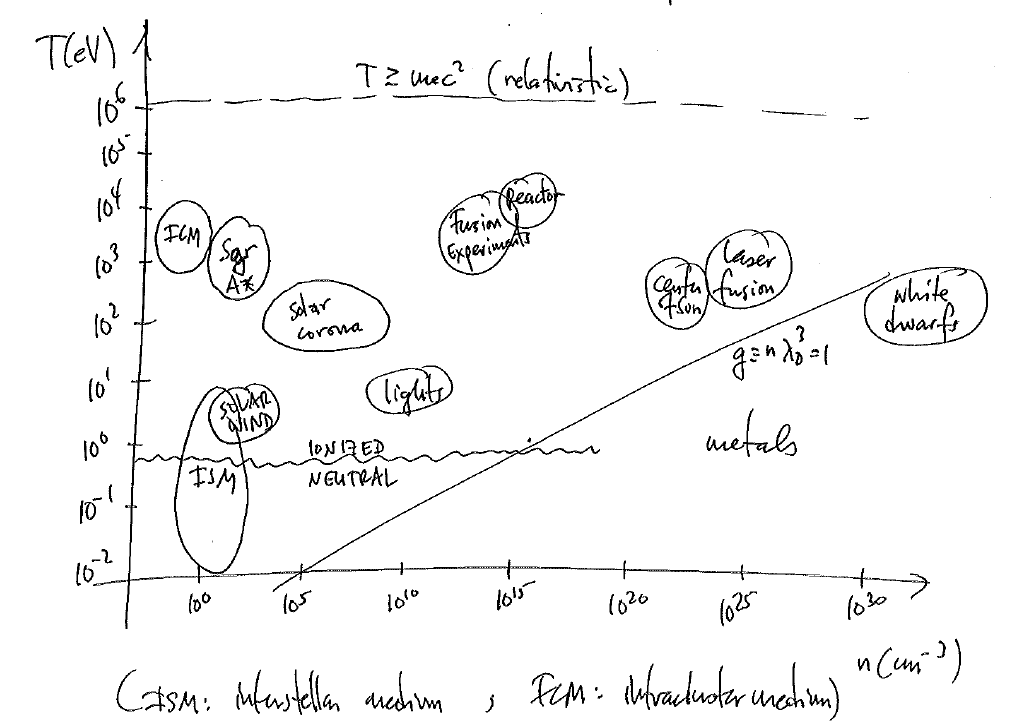
\includegraphics[width=0.8\textwidth]{scales.png}
  \caption{Scales of plasma physics}
  \label{fig:plasma}
\end{figure}

The one thing that is important is the line on the graph, which is the plasma
parameter which is defined as:
\begin{equation}
  \label{eq:1}
  g = n\lambda_D^3 = 1
\end{equation}
where $\lambda_D$ is the Debye length that is defined by the screening of the
charge in a plasma where
\begin{equation}
  \label{eq:1}
  \phi \sim \frac{1}{r}e^{-r/\lambda_D}
\end{equation}

The plasma parameter can be defined in various ways, and when we can treat
plasma as having collective behavior when $g \gg 1$:
\begin{equation}
  \label{eq:2}
  g \sim \frac{\text{KE}}{\text{PE}} \sim \frac{T}{e/\lambda_D} \sim \frac{\lambda_{mfp}}{\lambda_D} \gg 1
\end{equation}

In the table these are basically things that are interesting to us. SW refer to
the solar wind, which we can measure with spacecrafts. Other interesting media
we will see in following lectures are ICM (Inter-galactic medium), GC (Galactic
center), and ISM (Inter-stellar medium). The nice thing about the ISM is that
everything is about 1.

To get an idea of what the units mean, the Earth magnetic field is about
$0.5\,\mathrm{G}$. The thermal speed $v_{th,i}$ is a measure of the random
motion of particles
\begin{equation}
  \label{eq:3}
  v_{th,i} = \left( \frac{2T}{m_i} \right)^{1/2},\quad f \sim e^{-v^2/v_{th}^{2}}
\end{equation}

One more speed which is the Alfven speed
\begin{equation}
  \label{eq:4}
  v_A = \frac{B}{\sqrt{4\pi mn}}
\end{equation}
This is the speed that a disturbance propagates along the magnetic field. The
beta parameter $\beta_i$ is the ratio of the two velocities.

Now that we have defined what is a plasma, we need to talk about what is a
fluid. This is where the mean free path comes in $\lambda_{mfp}\sim
v_{th}\tau_\mathrm{col}$. This characterizes how often the particles scatter.
When this path is small like ISM the medium behaves like a fluid because the
distribution function looks very much like a Maxwellian. The larger this scale
gets you start to question whether this medium behaves like a fluid.

The last length scale is called $\rho_i$ which is $v_{th,i} / \Omega_i$ which is
the thermal speed divided by the gyro-frequency of the ion. This is the size of
a particle under gyration in a magnetic field. This scale is tiny compared to
most of other scales, which is characteristic of astrophysical plasmas. This
means the particles know about the magnetic field.

One more thing is the typical gyro-frequencies of particles. The table gives a
nice impression of the separation of scales for astrophysical situations.

Now we will just write down the equations for plasma. Lets fix some notations
first. $\varrho$ is different from $\rho$, where the later means charge density,
and former means $\Sigma_sm_sn_s$.

The MHD equations
\begin{align}
  \frac{\partial\varrho}{\partial t} + \nabla\cdot(\varrho \mathbf{u}) &= 0 \\
  \frac{dM}{dt} = -\int \nabla\cdot(\varrho \mathbf{u})\,dV &= -\oint \varrho \mathrm{u}\cdot d\mathbf{S} \\
  \varrho \left( \frac{\partial \mathbf{u}}{\partial t} + \mathbf{u}\cdot \nabla \mathbf{u} \right) = -\nabla P + \mathbf{g}\varrho + \frac{\mathbf{J}\times\mathbf{B}}{c}
\end{align}
The third equation is basically Newton's second law. The left hand side is the
comoving derivative which we can also write as $D \mathbf{u}/Dt$. The third term
in the rhs is what makes MHD MHD, because we have Lorentz force. This is
implicitly non-relativistic, $v/c\ll 1$.

Lets talk a bit about the Lorentz force. We can rewrite it as
\begin{equation}
  \label{eq:5}
  \frac{\mathbf{J}\times \mathbf{B}}{c} = \frac{(\nabla\times \mathbf{B}) \times \mathbf{B}}{4\pi} = \frac{\mathbf{B}\cdot \nabla\cdot \mathbf{B}}{4\pi} - \nabla \frac{B^2}{8\pi}
\end{equation}
the second term is like a pressure of the magnetic field.

One last equation we want to write down is the entropy equation
\begin{equation}
  \label{eq:6}
  \frac{Ds}{Dt} = \frac{P}{\gamma - 1}\frac{D \ln P e^{-\gamma}}{D t} = \dot{Q}
\end{equation}
If we have a incompressible fluid $\nabla\cdot \mathbf{u} = 0$ then it implies
$T = \text{const}$ in a fluid element.

One difficulty of the MHD arises from the vector derivative $\mathbf{u}\cdot
\nabla \mathbf{u}$. It is very easy to drop terms when doing vector analysis. In
cylindrical coordinates for example, when we decompose the terms we will get the
Coriolis force and the centrifugal force. The details are sketched in the notes.

Now we have Maxwell equations:
\begin{align}
  \nabla\cdot \mathbf{B} & = 0 \\
  \frac{\partial \mathbf{B}}{\partial t} &= -c\nabla\times \mathbf{E} = \nabla \times (\mathbf{u}\times \mathbf{B}) - \nabla\times(\eta \nabla\times \mathbf{B})
\end{align}
the last term is a way to abstract the electric field where we could take
$\mathbf{E} = \eta \mathbf{J}$, which is just Ohm's law. The last term is a way
to characterize resistive diffusion in the fluid. This term is not important
when the magnetic Reynolds number is high.

The first term can be expanded using vector analysis
\begin{equation}
  \label{eq:7}
  \frac{\partial \mathbf{B}}{\partial t} = \mathbf{B}\cdot \nabla \mathbf{u} - \mathbf{u}\cdot \nabla \mathbf{B} - \mathbf{B}\nabla\cdot \mathbf{u}
\end{equation}
There is also a last term but it is zero because $\nabla\cdot \mathbf{B} = 0$.
The first term is called ``stretching'', the second ``advection'', and the third
``compression''.

One thing we can do is take this form of the induction equation, and the
continuity equation and combine them. We then have
\begin{equation}
  \label{eq:8}
  \frac{D}{Dt}\frac{\mathbf{B}}{\varrho} = \frac{\mathbf{B}}{\varrho}\cdot \nabla \mathbf{u}
\end{equation}
This means that if we have a point $\mathbf{x}$ moving with velocity
$\mathbf{u}$, and another point $\mathbf{x} + \boldsymbol{\xi}$ moving with
$\mathbf{u}(\mathbf{x} + \boldsymbol{\xi})$ then we have
\begin{equation}
  \label{eq:9}
  \frac{D\boldsymbol{\xi}}{D t} \approx \boldsymbol{\xi}\cdot \nabla \mathbf{u}
\end{equation}
What this means is that fluid elements that lie on field lines initially will
remain on the field lines. This is called the Lindquist theorem, or ``flux freezing''.

We also have the Alfven theorem which states that, if we have some surface $S$
and there are some magnetic field lines that threads the surface with $\Phi =
\int \mathbf{B}\cdot d\mathbf{S}$. If the above equation is true then the flux
does not change with the flow of the fluid: $d\Phi/dt = 0$. The magnetic field
is ``frozen'' into the fluid and if the fluid moves, the lines moves with it.

Now lets come back to the Lorentz force. Remember we have
\begin{equation}
  \label{eq:10}
  \frac{\mathbf{J}\times \mathbf{B}}{c} = \frac{\mathbf{B}\cdot \nabla \mathbf{B}}{4\pi} - \nabla \frac{B^2}{8\pi} = -\nabla\cdot \left[ \frac{B^2}{8\pi}\mathbf{I} - \frac{\mathbf{B} \mathbf{B}}{4\pi} \right] = -\nabla \mathbf{M}
\end{equation}
where $\mathbf{M}$ is called the Maxwell stress tensor. The first term in the
bracket is diagonal, and the second term is the thing that introduces anisotropy
to the system by Lorentz force.

People usually say the first term is pressure and second term is tension but
that is not exactly true. Lets define $\hat{b} = \mathbf{B}/B$. We can write
the Lorentz force as
\begin{equation}
  \label{eq:11}
  \frac{B^2}{4\pi} \hat{b}\cdot\nabla \hat{b} - (\mathbf{I} - \hat{b} \hat{b})\cdot \nabla \frac{B^2}{8\pi}
\end{equation}
The first term is apparently perpendicular to the field line, and can be thought
of as the curvature force, as in the curved field line wants to be straightened.
The second term creates pressure towards the region where magnetic field is
small, wanting to spread out the field lines to be more even. This Lorentz force
is the fundamental difference between MHD and hydro, because magnetic field
doesn't want to be messed with, and it will direct the fluid.

An important part of MHD is the linear theory. We expand the quantities we are
interested in around an ``equilibrium'':
\begin{equation}
  \label{eq:12}
  \mathbf{u} = \mathbf{u}_0 + \delta \mathbf{u},\quad \varrho = \varrho_0 + \delta\varrho,\quad
  \mathbf{B} = \mathbf{B}_0 + \delta \mathbf{B},\quad P = P_0 + \delta P
\end{equation}
we use $\delta$ to denote Eulerian perturbation, and $\Delta$ to be Lagrangian
perturbation, where the former means the perturbation in lab frame, and the
latter means a change in the comoving frame of the fluid. Lets use Eulerian
perturbations for now for simplicity.

We have some equilibrium state denoted by suffix zero, and introduce some
perturbation to it, and in linear theory we just drop all the quadratic terms in
perturbation: $\delta^2 \longrightarrow 0$. In a homogeneous stationary plasma,
after we drop the quadratic terms we replace the perturbation with
\begin{equation}
  \label{eq:13}
  \delta \sim e^{-i\omega t + i\mathbf{k}\cdot \mathbf{r}}
\end{equation}
and then just do linear algebra.

One thing we can get out of this is called the Alfven wave. This is when
$\mathbf{k} = k_{\parallel}\hat{b}_0$. There is no change in $B_{\parallel}$ and
$\varrho$. The dispersion relation is very simple
\begin{equation}
  \label{eq:14}
  \omega = \pm k_{\parallel}v_A
\end{equation}
This is the fundamental building block of plasma perturbations.

We can also have compression waves in the fluid, which is like sound wave
\begin{equation}
  \label{eq:15}
  \omega = \pm k_{\parallel}c_s,\quad c_s = \left( \frac{\gamma P_0}{\varrho_{0}} \right)^{1/2}
\end{equation}
where $c_s$ is the speed of sound in the fluid.

We can also have a whole class of magnetic-sonic waves. Let $\mathbf{k} =
k_{\parallel}\hat{b}_0 + \mathbf{k}_{\perp}$. In regions with high $P$ and high
$B$, we have fast wave, and in regions with small $B$ we have slow wave. The
details of these waves are in the notes.

There is also an entropy mode where $\omega = 0$. That is all the mode we want
to talk about in MHD.

There is one more section which is called the Reduced MHD, but we are going to
skip it because of time. It is a useful technique for doing asymptotic
expansions.

When we wrote down all the equations we didn't talk about what was the velocity.
In MHD it is technically defined as
\begin{equation}
  \label{eq:16}
  \mathbf{u} = \frac{\sum_sm_sn_s\mathbf{u}_s}{\sum_sm_sn_s}
\end{equation}
which basically means center-of-mass velocity. In the limit of $n_i/n_n \ll 1$
the fluid velocity is governed by the neutral particle velocity which may not
make sense in MHD because neutral particles are not coupled to the magnetic
field. That is why we need to talk about multi-fluid MHD.

If we derive everything from the Vlasov equation, we can see that we have
continuity equation for every species
\begin{equation}
  \label{eq:17}
  \frac{\partial n_s}{\partial t} + \nabla\cdot \left( n_s\mathbf{u}_s \right) = 0
\end{equation}
and force equation for every species
\begin{equation}
  \label{eq:18}
  m_sn_s\frac{D \mathbf{u}_s}{D t_s} = -\nabla P_s + q_sn_s \left( \mathbf{E} + \frac{\mathbf{u}_s\times \mathbf{B}}{c} \right) + \mathbf{R}_s
\end{equation}
where the last term is the friction between species which add up to zero when we
sum all species. We also have the entropy equation for each species.

When we write down the induction equation for multi-fluid plasma, what should we
use as the plasma velocity $\mathbf{u}$? Suppose there is some frame where the
magnetic field is frozen, such that
\begin{equation}
  \label{eq:19}
  \frac{\partial \mathbf{B}}{\partial t} = \nabla \times \left( \mathbf{u}_f\times \mathbf{B} \right)
\end{equation}
for some $\mathbf{u}_{f}$. We can write it as
\begin{equation}
  \label{eq:20}
  \frac{\partial \mathbf{B}}{\partial t} = \nabla \times \left[ (\mathbf{u}_f - \mathbf{u}_{e}) \times \mathbf{B} + (\mathbf{u}_{e} - \mathbf{u}_{i})\times \mathbf{B} + (\mathbf{u}_{i} - \mathbf{u}_{n})\times \mathbf{B} + u_n\times \mathbf{B} \right]
\end{equation}
The three terms can be associated with different things. $u_f - u_{e}$ is what
we call Ohmic dissipation, which is like collisional resistivity. $u_i - u_n$ is
associated with Ambipolar diffusion, and $u_{i} - u_{e}$ is associated with Hall
effect. The Hall effect is related to nothing but the current $\mathbf{J} =
en_i(\mathbf{u}_{i} - \mathbf{u}_{e})$. Because $\mathbf{J} = \nabla\times
\mathbf{B}$ this introduces wave dispersion in MHD.

Lets come back to ambipolar diffusion. When do we expect $u_i$ and $u_n$ to
differ? This is related to the collision time scale between ions and neutral
particles
\begin{equation}
  \label{eq:21}
  \frac{u_i - u_n}{\tau_{ni}} \sim \frac{1}{\varrho_n}\left( \frac{\mathbf{J}\times \mathbf{B}}{c} \right)
\end{equation}
This is a kind of anisotropic diffusion for the magnetic field. It is useful to
re-derive the linear theory with these kind of drift speed between different
species of particles, and see what happens to different kinds of waves.

Where can we use these MHD? In solar wind people have used reduced MHD but
that's about it, because solar wind the fluid is not very collisional. In ICM
the collision is not quite strong enough. In GC the mean free path is about the
Bondi radius, especially if we keep going in near the black hole it is worse.
ISM has a cold and a warm phase, but both are pretty good for MHD.




\end{document}
